\documentclass[xcolor=table, aspectratio=169]{beamer}
\usepackage{beamerthemesplit}
\usepackage{wrapfig}
\usetheme{SPbGU}
\usepackage{pdfpages}
\usepackage{amsmath}
\usepackage{amssymb}
\usepackage{cmap}
\usepackage[T2A]{fontenc}
\usepackage[utf8]{inputenc}
\usepackage[english]{babel}
\usepackage{indentfirst}
\usepackage{tikz}
\usetikzlibrary{shapes,arrows,automata,positioning,quotes,backgrounds,decorations.text,decorations.pathmorphing}
\usepackage{multirow}
\usepackage[noend]{algpseudocode}
\usepackage{algorithm}
\usepackage{algorithmicx}
\usepackage{fancyvrb}
\usepackage[linguistics]{forest}
\usepackage{listings}
\usepackage{multicol}
\usepackage{comment}
\usepackage{xspace}
\usepackage{adjustbox}
\usepackage{makecell}
\usepackage{ stmaryrd }
\usepackage{ulem}


\newcommand{\backupbegin}{
   \newcounter{finalframe}
   \setcounter{finalframe}{\value{framenumber}}
}
\newcommand{\backupend}{
   \setcounter{framenumber}{\value{finalframe}}
}

\newcommand{\makenote}[1]{\hfill \footnotesize{#1}}
\newcommand{\strikeoutnote}[1]{\makenote{\strikethrough{#1}}}
\newcommand{\strikethrough}[1]{\sout{#1}}

\newcommand{\lststrikethrough}[1]{\ttfamily\sout{#1}}

\newcolumntype{A}{>{\hb@xt@\z@\bgroup\hss}r<{\egroup}}
\newcolumntype{B}{>{\hb@xt@\z@\bgroup}l<{\hss\egroup}}

\setbeamertemplate{itemize item}[circle]
\setbeamertemplate{enumerate items}[circle]

\lstdefinelanguage{ocanren}{
keywords={where, case, run, conde, fresh, let, match, with, when, class, type,
object, method, of, rec, repeat, until, while, \begin{comment}not,\end{comment} do, done, as, val, inherit,
new, module, sig, deriving, datatype, struct, if, then, else, open, private, virtual, include, success, failure,
true, false, mplus},
sensitive=true,
commentstyle=\small\itshape\ttfamily,
keywordstyle=\color{blue},
identifierstyle=\ttfamily,
basewidth={0.5em,0.5em},
columns=flexible,
mathescape=true,
escapechar=~,
fontadjust=true,
literate={fun}{{$\lambda$}}1 {function}{function}8 {->}{{$\to$}}3 {<-}{{$\leftarrow$}}3 {===}{{$\equiv$}}1 {=/=}{{$\not\equiv$}}1 {|>}{{$\triangleright$}}3 {\\/}{{$\vee$}}2 {/\\}{{$\wedge$}}2 {^}{{$\uparrow$}}1,
morecomment=[s]{(*}{*)},
 moredelim=**[is][\color{red}]{@!}{@}
}

\tikzstyle{processTree} = [
  ->,
  sibling distance=15em,
  scale=0.6,
  every node/.style = {
    shape=rectangle,
    rounded corners=0.05cm,
    draw,
    align=center,
    minimum size=5mm,
    scale=0.6,},
  %level 1/.style={sibling distance=100em}
  ]


\tikzstyle{program} = [
  draw=black,
  thick,
  rectangle,
  rounded corners=1pt,
  inner sep=5pt,
  inner ysep=5pt
  ]

\tikzstyle{goal} = [
  draw=black,
  rectangle,
  rounded corners=1pt,
  inner ysep=0pt,
  ]

\tikzstyle{input} = [
  draw=none,
  rectangle,
  rounded corners=1pt,
  inner sep=2pt,
  inner ysep=2pt,
  fill=green!10,
  minimum height=5mm
  ]


\tikzstyle{transparent} = [
  draw=none,
  inner ysep=3pt
  ]

\lstset{
language=ocanren
}


\DeclareMathOperator{\Term}{\mathcal{T}}
\DeclareMathOperator{\FlatTerm}{\mathcal{FT}}
\DeclareMathOperator{\Var}{\mathbf{Var}}
\DeclareMathOperator{\Cons}{\mathcal{C}}
\DeclareMathOperator{\Kan}{\mathcal{G}}
\DeclareMathOperator{\Fresh}{\mathbf{Fresh}}
\DeclareMathOperator{\Delay}{\mathbf{Delay}}
\DeclareMathOperator{\Cll}{\mathbf{Call}}
\DeclareMathOperator{\Def}{\mathcal{D}}
\DeclareMathOperator{\Base}{\mathbf{Base}}
\DeclareMathOperator{\Conj}{\mathbf{Conj}}
\DeclareMathOperator{\free}{\mathbf{free}}
\DeclareMathOperator{\ground}{\mathbf{ground}}
\DeclareMathOperator{\In}{\mathbf{In}}
\DeclareMathOperator{\Out}{\mathbf{Out}}
\DeclareMathOperator{\Fun}{\mathcal{F}}
\DeclareMathOperator{\Rtrn}{\mathbf{Return}}
\DeclareMathOperator{\Bind}{\mathbf{Bind}}
\DeclareMathOperator{\Match}{\mathbf{Match}}
\DeclareMathOperator{\Sum}{\mathbf{Sum}}
\DeclareMathOperator{\Guard}{\mathbf{Guard}}
\DeclareMathOperator{\Gen}{\mathbf{Gen}}
\DeclareMathOperator{\Stream}{\mathit{Stream}}
\DeclareMathOperator{\vars}{vars}
\DeclareMathOperator{\inmode}{\mathtt{I}}
\DeclareMathOperator{\outmode}{\mathtt{O}}
\DeclareMathOperator{\whatmode}{\mathtt{?}}
% \DeclareMathOperator{\inmode}{g \rightarrow g}
% \DeclareMathOperator{\outmode}{f \rightarrow g}
% \DeclareMathOperator{\mode1}{mode}
% \DeclareMathOperator{\Mode1}{\mathcal{M}}
\newcommand{\KanN}{\mathcal{K}^{N}}
\newcommand{\tran}[1]{\left\llbracket #1 \right\rrbracket}
\newcommand{\LIST}[1]{\left[ #1 \right]}
\renewcommand{\emptyset}{\varnothing}
\newcommand{\mk}{\textsc{miniKanren}\xspace}
\newcommand{\ocaml}{\textsc{OCaml}\xspace}
\newcommand{\haskell}{\textsc{Haskell}\xspace}
\renewcommand{\and}{$\&$\xspace}
\newcommand{\rel}[2]{\texttt{#1}$^o$ #2}
\newcommand{\subst}[1]{$\langle$#1$\rangle$}
\newcommand{\sem}[1]{\llbracket #1 \rrbracket}

\beamertemplatenavigationsymbolsempty

\title[Direction-Driven Functional Conversion]{Semi-Automated Direction-Driven Functional Conversion}
\institute[JetBrains Research]{
JetBrains Research, Programming Languages and Tools Lab

\vspace{1cm}

miniKanren workshop @ ICFP 2023
}

\author[Kate, Igor]{Kate Verbitskaia, Igor Engel, Daniil Berezun}

\date{08.09.2023}

\definecolor{orange}{RGB}{179,36,31}

\begin{document}
{
\begin{frame}[fragile]
   \begin{center}
      
\includegraphics[height=1.5cm]{pictures/jetbrainsResearch.pdf}
    \end{center}
  \titlepage
\end{frame}
}

\begin{frame}[fragile]
  \frametitle{Relational Programming}
\begin{center}
Nondeterminism
\end{center}

\begin{center}
Completeness of search
\end{center}

\begin{center}
One relation to solve many problems
\end{center}
\end{frame}

\begin{frame}[fragile]
  \frametitle{Relational Interpreters for Search Problems}
  \begin{center}

Given a function


\begin{figure}[!t]
  \centering
  \begin{minipage}{0.55\textwidth}
    \begin{lstlisting}[frame=tb]
 eval (Conj x y) =
   eval x && eval y
 ...
    \end{lstlisting}
  \end{minipage}
\end{figure}


Generate a \mk relation
\begin{figure}[!t]
  \centering
  \begin{minipage}{0.75\textwidth}
    \begin{lstlisting}[frame=tb]
 eval$^o$ fm u = fresh (x y v w)
     (fm === Conj x y /\ 
      and$^o$ v w u /\ 
      eval$^o$ x v /\ 
      eval$^o$ y w);
     ...
    \end{lstlisting}
  \end{minipage}
\end{figure}


Run it to solve a search problem:
\lstinline{run q (eval$^o$ q true)}
\end{center}

\end{frame}


\begin{frame}[fragile]
  \frametitle{Principal Directions of \mk Relations}
\begin{center}
  Every argument of a relation can be either input (\lstinline{I}) or output (\lstinline{O})

\vfill

  \strikeoutnote{Partially known terms such as \lstinline{(Cons _.0 Nil)}}
\end{center}

\vfill

\begin{center}
  The 8 directions of the addition relation \lstinline{add$^o$ x y z}:
\end{center}

\begin{center}
\begin{tabular}{rll}
  \emph{Forward}   & \lstinline|add$^o$ I I O| & addition      \\
  \emph{Backward}  & \lstinline|add$^o$ O O I| & decomposition \\
  \emph{Predicate} & \lstinline|add$^o$ I I I| &               \\
  \emph{Generator} & \lstinline|add$^o$ O O O| &               \\
                   & \lstinline|add$^o$ I O I| & subtraction   \\
                   & \lstinline|add$^o$ O I I| & subtraction   \\
                   & \lstinline|add$^o$ O I O| &               \\
                   & \lstinline|add$^o$ I O O| &
\end{tabular}
\end{center}
\end{frame}


\begin{frame}[fragile]
  \frametitle{Each Direction is a Function}
\end{frame}

\begin{frame}[noframenumbering]
  \frametitle{Each Direction is a Function (Kind of)}
\begin{center}
Functions

\vfill

\begin{tabular}{rcl}
 ~~~ \emph{Forward} & \lstinline|add$^{o\,\,}$ I I O| & addition    \\
                    & \lstinline|add$^{o\,\,}$ I O I| & subtraction \\
                    & \lstinline|add$^{o\,\,}$ O I I| & subtraction \\
  \emph{Predicate}  & \lstinline|add$^{o\,\,}$ I I I| &
\end{tabular}
\end{center}

\vfill

\begin{center}
Relations

\vfill

\begin{tabular}{rcl}
 ~~~~~ \emph{Backward}  & \lstinline|add$^{o\,\,}$ O O I| & decomposition \\
       \emph{Generator} & \lstinline|add$^{o\,\,}$ O O O| &               \\
                        & \lstinline|add$^{o\,\,}$ O I O| &               \\
                        & \lstinline|add$^{o\,\,}$ I O O| &
\end{tabular}
\end{center}

\makenote{Relations are functions which return multiple answers}

\end{frame}

\begin{frame}[fragile]
  \frametitle{\mk Comes with an Overhead}
  \begin{center}
    Unifications
  \end{center}

  \begin{center}
    Occurs-check
  \end{center}

  \begin{center}
    Scheduling complexity
  \end{center}
\end{frame}

\begin{frame}[fragile]
  \frametitle{Functional Conversion}
\begin{center}
  Given a relation and a principal direction, construct a functional program that generates the same answers as \mk would
\end{center}

\vfill

\begin{center}
  Preserve the completeness of the search
\end{center}

\vfill

\begin{center}
Both inputs and outputs are expected to be ground
\end{center}
\end{frame}

\lstset{basicstyle=\small}

\begin{frame}[fragile]
  \frametitle{Example: Addition in the Forward Direction}
\begin{columns}
  \begin{column}[t]{0.49\textwidth}
    \begin{figure}[!t]
  \centering
  \begin{minipage}{0.7\columnwidth}
    \begin{lstlisting}[frame=tb]
 let rec add$^o$ x y z = conde [
   (x === O /\ y === z);
   (fresh (x$_1$ z$_1$)
     (x === S x$_1$ /\
      add$^o$ x$_1$ y z$_1$ /\
      z === S z$_1$) ) ]
    \end{lstlisting}
  \end{minipage}
\end{figure}
  \end{column}
  \begin{column}[t]{0.49\textwidth}
    \begin{figure}[!t]
  \centering
  \begin{minipage}{\columnwidth}
    \begin{lstlisting}[frame=tb]
addIIO :: Nat -> Nat -> Nat
addIIO x y =
  case x of
    O -> y
    S x$_1$ -> S (addIIO x$_1$ y)
    \end{lstlisting}
  \end{minipage}
\end{figure}

  \end{column}
\end{columns}
\end{frame}

\begin{frame}[fragile]
  \frametitle{Example: Addition in the Forward Direction}
    \begin{figure}[!t]
  \centering
  \begin{minipage}{0.7\columnwidth}
    \begin{lstlisting}[frame=tb]
addoIIO x0 x1 = 
  msum [do {guard (x0 == O);
            let {x2 = x1};
            return x2},
        do {x3 <- case x0 of
              {S y3 -> return y3; 
               _ -> mzero};
            x4 <- addoIIO x3 x1;
            let {x2 = S x4};
            return x2}]
    \end{lstlisting}
  \end{minipage}
\end{figure}
 
\end{frame}

\begin{frame}[fragile]
  \frametitle{Addition in the Backward Direction: Nondeterminism}
\begin{columns}
  \begin{column}[t]{0.49\textwidth}
    \begin{figure}[!t]
  \centering
  \begin{minipage}{0.7\columnwidth}
    \begin{lstlisting}[frame=tb]
 let rec add$^o$ x y z = conde [
   (x === O /\ y === z);
   (fresh (x$_1$ z$_1$)
     (x === S x$_1$ /\
      add$^o$ x$_1$ y z$_1$ /\
      z === S z$_1$) ) ]
    \end{lstlisting}
  \end{minipage}
\end{figure}
  \end{column}
  \begin{column}[t]{0.49\textwidth}
    \begin{figure}[!t]
  \centering
  \begin{minipage}{0.9\columnwidth}
    \begin{lstlisting}[frame=tb,language=ocanren1]
addOOI $::$ Nat -> Stream (Nat, Nat)
addOOI z =
  return (O, z) <$\mid$>
  case z of
    O -> Empty
    S z$_1$ -> do
      (x$_1$, y) <- addOOI z$_1$
      return (S x$_1$, y)
    \end{lstlisting}
  \end{minipage}
\end{figure}

  \end{column}
\end{columns}
\end{frame}

\begin{frame}[fragile]
  \frametitle{Free Variables in Answers: Generators}
\begin{columns}
  \begin{column}[t]{0.49\textwidth}
    \begin{figure}[!t]
  \centering
  \begin{minipage}{0.7\columnwidth}
    \begin{lstlisting}[frame=tb]
 let rec add$^o$ x y z = conde [
   (x === O /\ y === z);
   (fresh (x$_1$ z$_1$)
     (x === S x$_1$ /\
      add$^o$ x$_1$ y z$_1$ /\
      z === S z$_1$) ) ]
    \end{lstlisting}
  \end{minipage}
\end{figure}
  \end{column}
  \begin{column}[t]{0.49\textwidth}
    \begin{figure}[!t]
  \centering
  \begin{minipage}{\columnwidth}
    \begin{lstlisting}[label={add_x},
                      %  caption={Function for \lstinline{addo in out out} direction},
                       captionpos=b,
                       frame=tb]
addX :: Nat -> Stream (Nat, Nat)
addX x = case x of
           O -> do
             z <- genNat
             return (z, z)
           S x' -> do
             (y, z') <- addX x'
             return (y, S z')

genNat :: Stream Nat
genNat = Mature O (S <$\$$> genNat)
    \end{lstlisting}
  \end{minipage}
\end{figure}
  \end{column}
\end{columns}
\end{frame}

% \begin{frame}[fragile]
%   \frametitle{Predicates}
% \begin{columns}
%   \begin{column}[t]{0.48\textwidth}
%     \begin{figure}[!t]
  \centering
  \begin{minipage}{0.7\columnwidth}
    \begin{lstlisting}[frame=tb]
 let rec add$^o$ x y z = conde [
   (x === O /\ y === z);
   (fresh (x$_1$ z$_1$)
     (x === S x$_1$ /\
      add$^o$ x$_1$ y z$_1$ /\
      z === S z$_1$) ) ]
    \end{lstlisting}
  \end{minipage}
\end{figure}
%   \end{column}
%   \begin{column}[t]{0.5\textwidth}
%     \begin{figure}[!t]
  \centering
  \begin{minipage}{\columnwidth}
    \begin{lstlisting}[frame=tb]
 addIII $::$ Nat -> Nat -> Nat -> Stream ()
 addIII x y z =
   case x of
     O | y == z -> return ()
       | otherwise -> Empty
     S x$_1$ ->
       case z of
         O -> Empty
         S z$_1$ -> addIII x$_1$ y z$_1$
    \end{lstlisting}
  \end{minipage}
\end{figure}
%   \end{column}
% \end{columns}
% \end{frame}

\begin{frame}[fragile]
  \frametitle{Conversion Scheme}

\begin{center}
  Normalization
\end{center}

\begin{center}
  Mode analysis
\end{center}

\begin{center}
  Functional conversion
\end{center}
\end{frame}


\begin{frame}[fragile]
  \frametitle{Normalization: Flat Term}
\begin{center}
Flat terms: a variable or a constructor with \emph{distinct} variables for arguments
\end{center}

  \[  \FlatTerm_{V} = V \cup \{\Cons \, x_0 \ldots \, x_{k} \mid x_{j}\in V, x_j - distinct \} \]

\vfill

\begin{center}
\begin{tabular}{rcl}
 $C\left( x_1, x_2 \right) \equiv C\left( C\left( y_1, y_2 \right), y_3 \right)$ & $\iff$ &  $x_1 \equiv C\left( y_1, y_2 \right) \land x_2 \equiv y_3$ \\
 $C\left( C\left( x_1, x_2 \right), x_3 \right) \equiv C\left( C\left( y_1, y_2 \right), y_3 \right)$ & $\iff$ & $x_1 \equiv y_1 \land x_2 \equiv y_2 \land x_3 \equiv y_3$ \\
 $x \equiv C\left( y, y \right)$ & $\iff$ & $x \equiv C\left( y_1, y_2 \right)\land y_1 \equiv y_2$
\end{tabular}
\end{center}

\vfill

\strikeoutnote{Constructors inside constructors}

\strikeoutnote{Repeating variables}

\end{frame}

\begin{frame}[fragile]
  \frametitle{Normalization: Goal}
\begin{center}
\begin{tabular}{rclll}
$\KanN_{V}$ & $=$ & $c_1 \vee \ldots \vee c_{n}$ & $c_{i}\in \Conj_{V}$ & normal form \\
$\Conj_{V}$ & $=$ & $g_1 \wedge \ldots \wedge g_n$ & $ g_{i}\in \Base_{V}$ & normal conjunction \\
$\Base_{V}$ & $=$ & $V \equiv \FlatTerm_{V}$ & & flat unification \\
            & $\mid$ & $R \, x_1 \ldots \, x_{k} $ & $ x_{j}\in V, x_j - distinct$ & flat call \\
\end{tabular}
\end{center}


\vfill

\strikeoutnote{Disjunctions within conjunctions}

\strikeoutnote{Empty disjunctions and conjunctions}

\strikeoutnote{Constructors as arguments of relation calls}

\end{frame}


\begin{frame}[fragile]
  \frametitle{Mode of a Variable}
\begin{center}
\begin{tabular}{rll}
  \emph{Ground} term & no fresh variables & \lstinline|Cons O (Cons (S O) Nil)| \\
  \emph{Free} variable & a fresh variable & \lstinline|_.0|
\end{tabular}

\vfill

Once we know that a variable is \emph{ground}, it stays \emph{ground} in later conjuncts
\end{center}

\vfill

\begin{center}
Mode of a variable: mapping between its instantiations

\vfill

\begin{tabular}{rl}
  Mode \lstinline|I|: & \lstinline|ground| $\rightarrow$ \lstinline|ground| \\
  Mode \lstinline|O|: & \lstinline|free| $\rightarrow$ \lstinline|ground|
\end{tabular}
\end{center}

\vfill

\hfill \footnotesize Mercury uses more complicated modes

\end{frame}

\begin{frame}[fragile]
  \frametitle{Modded Goal}
  \begin{center}
Assign mode to every variable, make sure they are consistent
  \end{center}
\end{frame}

\begin{frame}[fragile]
  \frametitle{Modded Unification Types}

\begin{center}
\begin{tabular}{rl}
  assignment & $x^{\outmode} \equiv \Term^{\inmode} $ \\
             & $x^{\inmode}  \equiv y^{\outmode}    $ \\
  guard      & $x^{\inmode}  \equiv \Term^{\inmode} $ \\
  match      & $x^{\inmode}  \equiv \Term           $ \\
  generator  & $x^{\outmode} \equiv \Term           $
\end{tabular}
\end{center}

\hfill \footnotesize $\Term$ contains both $g$ and $f$ variables
\end{frame}

\begin{frame}[fragile]
  \frametitle{Mode Inference: Initialization }


\begin{center}
\begin{tabular}{rcl}
  Input variables:  & $\mathtt{I}$ & g $\rightarrow$ g \\
  Output variables: & $\mathtt{O}$ & f $\rightarrow$ g \\
  Other variables:  & $\mathtt{?}$ & f $\rightarrow$ ?
\end{tabular}
\end{center}

\vfill

\begin{figure}[!t]
  \centering
  \begin{minipage}{\columnwidth}
    \begin{lstlisting}[frame=tb]
let rec add$^o$ x$^{g \to g}$ y$^{g \to g}$ z$^{f \to g}$ = conde
  (x$^{g \to g}$  ===    O /\ y$^{g \to g}$ ===     z$^{f \to g}$);
  (x$^{g \to g}$ ===     S x$_1^{f \to ?}$ /\
   add$^o$ x$_1^{f \to ?}$ y$^{g \to g}$ z$_1^{f \to ?}$ /\
   z$^{f \to g}$ ===     S z$_1^{f \to ?}$)
    \end{lstlisting}
  \end{minipage}
\end{figure}
\end{frame}

\begin{frame}[fragile]
  \frametitle{Mode Inference: Disjunction }

\begin{center}
Run inference on each disjunct independently
\end{center}

\begin{columns}
  \begin{column}[t]{0.15\textwidth}
  \end{column}
  \begin{column}[t]{0.34\textwidth}
    \begin{figure}[!t]
  \centering
  \begin{minipage}{0.65\columnwidth}
    \begin{lstlisting}[frame=tb]
 x$^{\inmode}$  === O /\ y$^{\inmode}$ ===  z$^{\outmode}$
    \end{lstlisting}
  \end{minipage}
\end{figure}
  \end{column}
  \begin{column}[t]{0.34\textwidth}
    \begin{figure}[!t]
  \centering
  \begin{minipage}{0.55\columnwidth}
    \begin{lstlisting}[frame=tb]
 x$^{\inmode}$ ===  S x$_1^{\whatmode}$ /\
 add$^o$ x$_1^{\whatmode}$ y$^{\inmode}$ z$_1^{\whatmode}$ /\
 z$^{\outmode}$ ===  S z$_1^{\whatmode}$
    \end{lstlisting}
  \end{minipage}
\end{figure}
  \end{column}
  \begin{column}[t]{0.15\textwidth}
  \end{column}
\end{columns}
\end{frame}


\begin{frame}[fragile]
  \frametitle{Mode Inference: Unification}
\begin{center}
Propagate the groundness information according to the 4 types of modded unifications
\end{center}

\begin{columns}
  \begin{column}[t]{0.3\textwidth}
  \end{column}
  \begin{column}[t]{0.2\textwidth}
    \begin{figure}[!t]
  \centering
  \begin{minipage}{0.65\columnwidth}
    \begin{lstlisting}[frame=tb]
 x$^{\inmode}$ ===  S x$_1^{\whatmode}$
    \end{lstlisting}
  \end{minipage}
\end{figure}
  \end{column}
  \begin{column}[t]{0.2\textwidth}
    \begin{figure}[!t]
  \centering
  \begin{minipage}{0.65\columnwidth}
    \begin{lstlisting}[frame=tb]
 x$^{\inmode}$ ===  S x$_1^{\outmode}$
    \end{lstlisting}
  \end{minipage}
\end{figure}
  \end{column}
  \begin{column}[t]{0.3\textwidth}
  \end{column}
\end{columns}

\begin{columns}
  \begin{column}[t]{0.3\textwidth}
  \end{column}
  \begin{column}[t]{0.2\textwidth}
    \begin{figure}[!t]
  \centering
  \begin{minipage}{0.65\columnwidth}
    \begin{lstlisting}[frame=tb]
 z$^{\outmode}$ ===  S z$_1^{\whatmode}$
    \end{lstlisting}
  \end{minipage}
\end{figure}
  \end{column}
  \begin{column}[t]{0.2\textwidth}
    \begin{figure}[!t]
  \centering
  \begin{minipage}{0.65\columnwidth}
    \begin{lstlisting}[frame=tb]
 z$^{\outmode}$ ===  S z$_1^{\outmode}$
    \end{lstlisting}
  \end{minipage}
\end{figure}
  \end{column}
  \begin{column}[t]{0.3\textwidth}
  \end{column}
\end{columns}

\end{frame}

\begin{frame}[fragile]
  \frametitle{Mode Inference: Conjunction}
\begin{center}
Pick a conjunct according to the priority, propagate groundness
\end{center}

\vfill

\begin{center}
  \begin{minipage}{0.4\textwidth}
    \begin{enumerate}
      \item Guard
      \item Assignment
      \item Match
      \item Call with some ground arguments
      \item Unification-generator
      \item Call with all free arguments
    \end{enumerate}
  \end{minipage}
\end{center}


\end{frame}

\begin{frame}[fragile]
  \frametitle{Mode Inference: Conjunction}
\begin{columns}
  \begin{column}[t]{0.33\textwidth}
    \begin{figure}[!t]
  \centering
  \begin{minipage}{\columnwidth}
    \begin{lstlisting}[label={add},
                      %  caption={Addition relation},
                       captionpos=b,
                       frame=tb]
  x$^{g \to g}$ ===     S x$_1^{f \to ?}$ /\
  add$^o$ x$_1^{f \to ?}$ y$^{g \to g}$ z$_1^{f \to ?}$ /\
  z$^{g \to g}$ ===     S z$_1^{f \to ?}$
    \end{lstlisting}
  \end{minipage}
\end{figure} \pause
  \end{column}
  \begin{column}[t]{0.33\textwidth}
    \begin{figure}[!t]
  \centering
  \begin{minipage}{\columnwidth}
    \begin{lstlisting}[label={add},
                      %  caption={Addition relation},
                       captionpos=b,
                       frame=tb]
  (((x, g->g) === S (x', f->g) /\
    add$^o$ (x', f->g) (y, g->g) (z', f->?) /\
    (z,f->g) === S (z', f->?)))
    \end{lstlisting}
  \end{minipage}
\end{figure} \pause
  \end{column}
  \begin{column}[t]{0.33\textwidth}
    \begin{figure}[!t]
  \centering
  \begin{minipage}{0.57\columnwidth}
    \begin{lstlisting}[frame=tb]
 x$^{\inmode}$ ===  S x$_1^{\outmode}$ /\
 add$^o$ x$_1^{\inmode}$ y$^{\inmode}$ z$_1^{\outmode}$ /\
 z$^{\outmode}$ ===  S z$_1^{\inmode}$
    \end{lstlisting}
  \end{minipage}
\end{figure}
  \end{column}
\end{columns}
\end{frame}

\begin{frame}[fragile]
  \frametitle{Order in Conjunctions: Slow Version}

\begin{columns}
  \begin{column}[t]{0.4\textwidth}
    \begin{figure}[!t]
  \centering
  \begin{minipage}{\columnwidth}
    \begin{lstlisting}[label={mult},
                      %  caption={Multiplication relation},
                       captionpos=b,
                       frame=tb]
let rec mult$^o$ x y z = conde [
  ...
  (fresh (x' r')
    (x === S x') /\
    (add y r' z) /\
    (mult x' y r')
  )]
    \end{lstlisting}
  \end{minipage}
\end{figure}

  \end{column}
  \begin{column}[t]{0.55\textwidth}
    \begin{figure}[!t]
  \centering
  \begin{minipage}{\columnwidth}
    \begin{lstlisting}[label={mult_slow}, caption={Inefficient implementation of \lstinline{multo in in out} direciton}, captionpos=b, frame=tb]
multXY' :: Nat -> Nat -> Stream Nat
multXY' O     y     = return O
multXY' x     O     = return O
multXY' (S O) y     = return y
multXY' x     (S O) = return x
multXY' (S x') y    = do
  (r', r) <- addX y
  multXYZ x' y r'
  return r

multXYZ :: Nat -> Nat -> Nat -> Stream ()
multXYZ O      y     O = return ()
multXYZ x      O     O = return ()
multXYZ (S O)  y     z | y == z = return ()
multXYZ x      (S O) z | x == z = return ()
multXYZ (S x') y     z = do
  z' <- multXY' x' y
  addXYZ y z' z
multXYZ _ _ _ = Empty
    \end{lstlisting}
  \end{minipage}
\end{figure}

  \end{column}
\end{columns}

\begin{center}
  Premature grounding of \lstinline{z$_1$} leads to the \emph{generate-and-test} behavior
\end{center}

\end{frame}


\begin{frame}[fragile]
  \frametitle{Order in Conjunctions: Faster Version}

\begin{columns}
  \begin{column}[t]{0.4\textwidth}
    \begin{figure}[!t]
  \centering
  \begin{minipage}{\columnwidth}
    \begin{lstlisting}[label={mult},
                      %  caption={Multiplication relation},
                       captionpos=b,
                       frame=tb]
let rec mult$^o$ x y z = conde [
  ...
  (fresh (x' r')
    (x === S x') /\
    (add y r' z) /\
    (mult x' y r')
  )]
    \end{lstlisting}
  \end{minipage}
\end{figure}

  \end{column}
  \begin{column}[t]{0.55\textwidth}
    \begin{figure}[!t]
  \centering
  \begin{minipage}{0.8\columnwidth}
    \begin{lstlisting}[frame=tb]
 multIIO $::$ Nat -> Nat -> Stream Nat
 multIIO (S x$_1$) y = do
   r$_1$ <- multIIO x$_1$ y
   addIIO y r$_1$
 ...
    \end{lstlisting}
  \end{minipage}
\end{figure}

  \end{column}
\end{columns}
\end{frame}

\begin{frame}[fragile]
  \frametitle{Functional Conversion: Intermediate Language}
\begin{center}
\begin{tabular}{lcll}
    $\Fun_{V}$ & $=$ &  $\Rtrn \LIST{\Term_{V}}$ & return a tuple of terms\\
               & $\mid$ &  $\Match_{V} \left( \Term_{V}, \Fun_{V} \right)$& match a variable against a pattern\\
               & $\mid$ & $\Bind\LIST{\left(\LIST{V}, \Fun_{V}\right)} $ & monadic bind on streams\\
               & $\mid$ & $\Sum\LIST{\Fun_{V}}$ & concatenation of streams\\
               & $\mid$ & $\Guard\left( V, V \right)$ & equality check\\
               & $\mid$ & $\Gen_{G}$ & generator\\
               & $\mid$ & $R_{i}(\LIST{V}, \LIST{G})$ & function call
\end{tabular}
\end{center}
\end{frame}

\begin{frame}[fragile]
  \frametitle{Functional Conversion into Intermediate Language}
\begin{center}
\begin{tabular}{rcl}
  Disjunction   & $\rightarrow$ & $\Sum\LIST{\Fun_{V}}$ \\ && \\
  Conjunction   & $\rightarrow$ & $ \Bind\LIST{\left(\LIST{V}, \Fun_{V}\right)}$ \\ && \\
  Relation call & $\rightarrow$ & $ R_{i}(\LIST{V}, \LIST{G})$ \\ && \\
  Unification   & $\rightarrow$ & $\Rtrn \LIST{\Term_{V}}$ \\
                & $|$           & $\Match_{V} \left( \Term_{V}, \Fun_{V} \right)$ \\
                & $|$           & $\Guard\left( V, V \right)$ \\
                & $|$           & $\Gen_{G}$
\end{tabular}
\end{center}
\end{frame}

\begin{frame}[fragile]
  \frametitle{Functional Conversion: Generators}
\begin{center}
  In the untyped miniKanren it is only possible to generate \emph{all terms}
\end{center}

\vfill

\begin{center}
  Instead pass generators to functions as additional arguments


  It is up to the user what generator to pass
\end{center}

\begin{figure}[!t]
  \centering
  \begin{minipage}{0.59\columnwidth}
    \begin{lstlisting}[frame=tb]
 addIOO $::$ Nat -> Stream Nat -> Stream (Nat, Nat)
 addIOO x gen$_z$ =
   case x of
     O -> do
       z <- gen$_z$
       return (z, z)
     S x$_1$ -> do
       (y, z$_1$) <- addIOO x$_1$ gen$_z$
       return (y, S z$_1$)
    \end{lstlisting}
  \end{minipage}
\end{figure}

\end{frame}

\begin{frame}[fragile]
  \frametitle{Functional Conversion: Generators}
\begin{center}
We pass a generator for every variable in \emph{rhs} of a unification-generator
\end{center}

\begin{center}
Generators used in calls should be passed to the parent function
\end{center}

\begin{center}
In a typed version, it should be possible to automatically derive generators from types
\end{center}

    \begin{figure}[!t]
  \centering
  \begin{minipage}{\columnwidth}
    \begin{lstlisting}[label={mult_x_gen},
                      %  caption={Efficient implementation of \lstinline{multo in in out} direciton},
                       captionpos=b,
                       frame=tb]
multOIO :: Nat -> Stream Nat -> Stream Nat
multOIO y gen_add$_z$ =
  return (O, O) `mplus`
  do
    (z$_1$, z) <- addIOO y gen_add$_z$
    x <- muloOII y z$_1$
    return (S x, z)
    \end{lstlisting}
  \end{minipage}
\end{figure}

\end{frame}

\begin{frame}[fragile]
  \frametitle{Functional Conversion into the Target Languages}
\begin{columns}
  \begin{column}[t]{0.45\textwidth}

\begin{center}
  \haskell
\end{center}

\begin{center}
  TemplateHaskell to generate code
\end{center}

\begin{center}
  Stream monad
\end{center}

\begin{center}
  do-notation
\end{center}

\begin{center}

\end{center}

  \end{column}
  \begin{column}[t]{0.45\textwidth}
\begin{center}
  \ocaml
\end{center}
\begin{center}
  Hand-crafted (not so) pretty-printer
\end{center}

\begin{center}
  Stream monad
\end{center}

\begin{center}
  let*
\end{center}

\begin{center}
  Taking extra care to ensure laziness
\end{center}

  \end{column}
\end{columns}

\end{frame}


\begin{frame}[fragile]
  \frametitle{Evaluation}
  \begin{center}
    We converted relational interpreters and measured execution time

\vfill

  \begin{minipage}{0.65\textwidth}
    \begin{itemize}
      \item Logic formulas generation
      \begin{itemize}
        \item Inverse computation of an evaluator of logic formulas
        \item Generating formulas which evaluate to \lstinline{true}
      \end{itemize}
      \item Multiplication relation
      \begin{itemize}
        \item Forward direction: multiplication
        \item Backward direction: division
        \item Generation
      \end{itemize}
    \end{itemize}
  \end{minipage}
\end{center}



\end{frame}

\begin{frame}[fragile]
  \frametitle{Generation of Logic Formulas: \lstinline[basicstyle=\Large]{evalo  [true; false; true] q true}}
  \begin{center}
    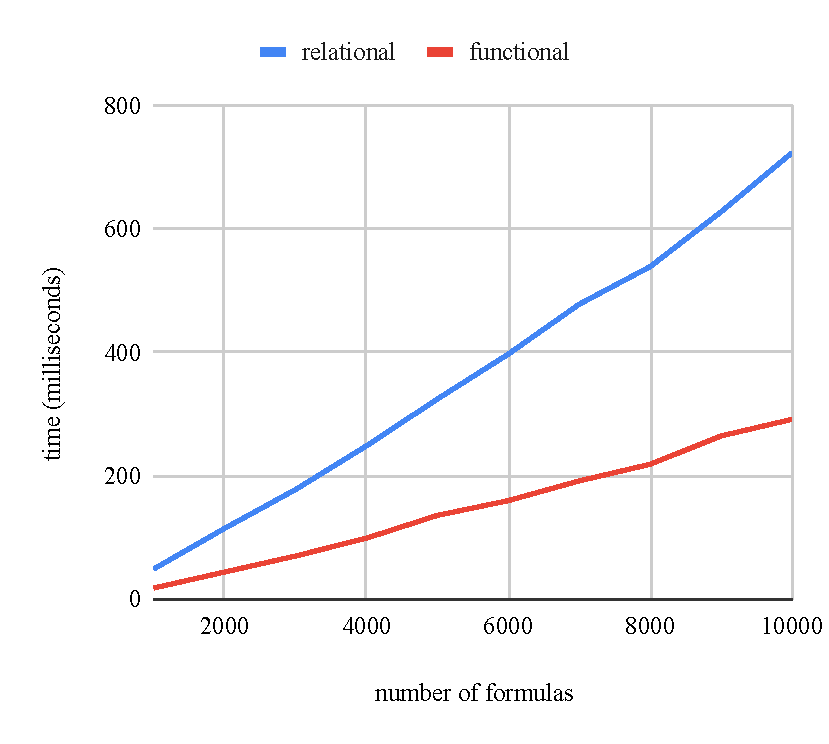
\includegraphics[height=0.85\textheight]{figures/propIOI.pdf}
  \end{center}
\end{frame}


\begin{frame}[fragile]
  \frametitle{Multiplication: \lstinline[basicstyle=\Large]{mulo n 10 q}}
  \begin{center}
    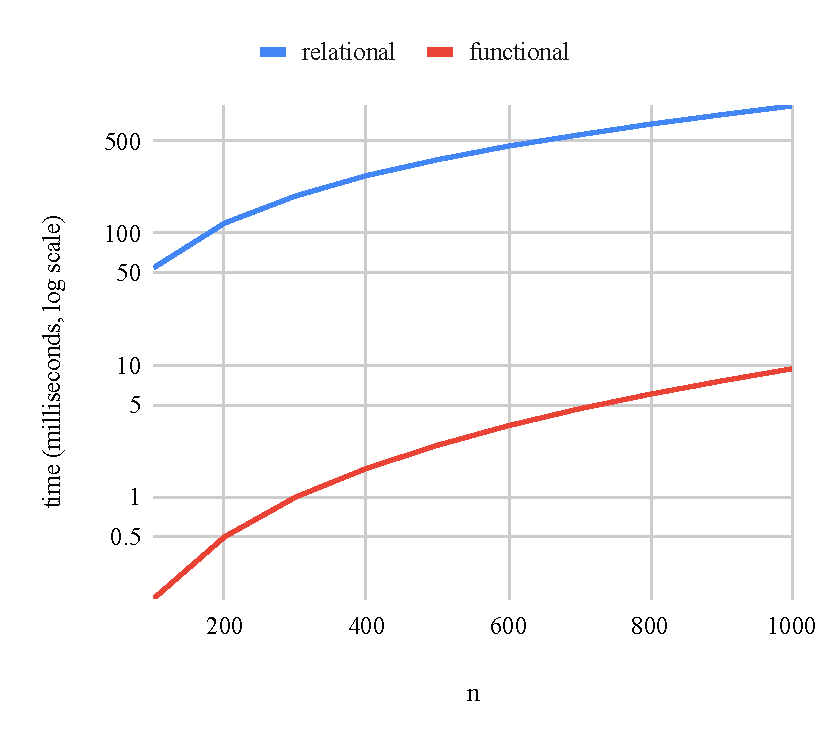
\includegraphics[height=0.85\textheight]{figures/muloIIO.pdf}
  \end{center}
\end{frame}


\begin{frame}[fragile]
  \frametitle{Division: \lstinline[basicstyle=\Large]{mulo (n/10) q n}}
  \begin{center}
    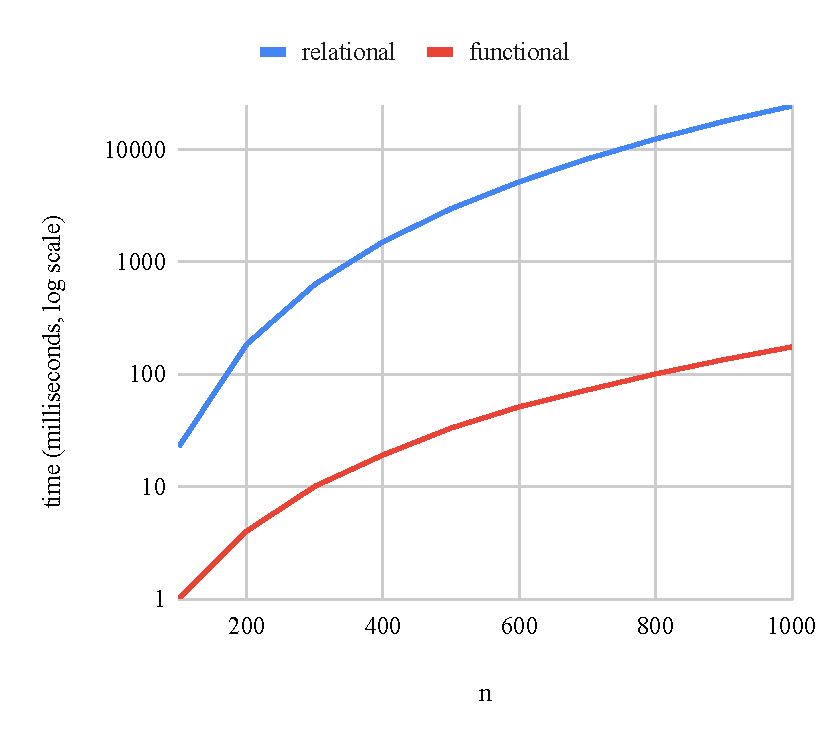
\includegraphics[height=0.85\textheight]{figures/muloIOI.pdf}
  \end{center}
\end{frame}

\begin{frame}[fragile]
  \frametitle{Multiplication Generation: \lstinline[basicstyle=\Large]{take n (mulo 10 q r)}}
  \begin{center}
    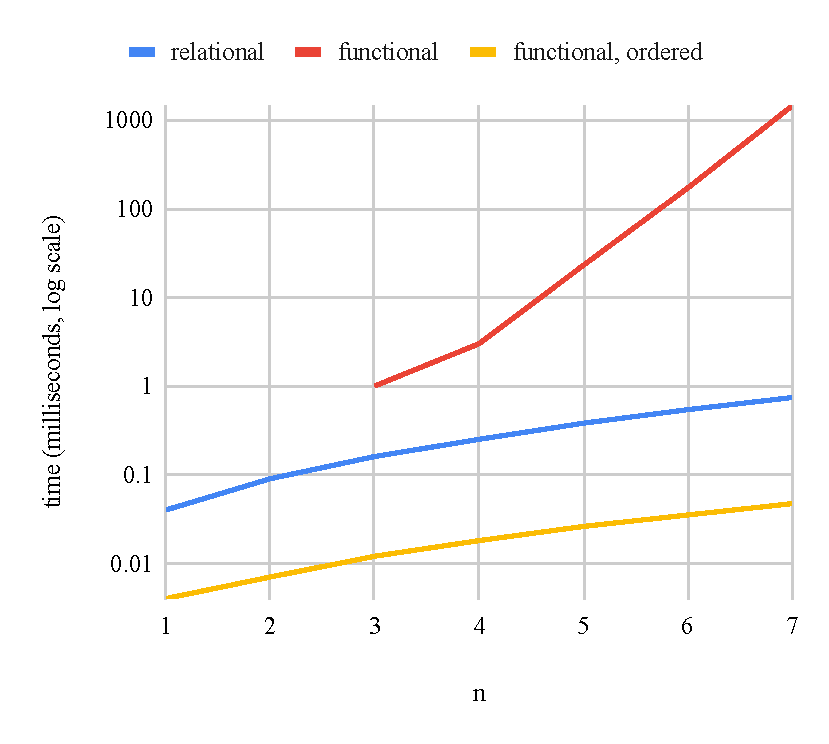
\includegraphics[height=0.85\textheight]{figures/muloIOO.pdf}
  \end{center}
\end{frame}


\begin{frame}[fragile]
  \frametitle{\lstinline[basicstyle=\Large]{Maybe} for Semi-Determinism}
\begin{center}
  \begin{minipage}{0.43\textwidth}
    \begin{figure}[!t]
  \centering
  \begin{minipage}{\columnwidth}
    \begin{lstlisting}[frame=tb]
muloOII :: Nat -> Nat -> Stream Nat
muloOII x1 x2 = zero `mplus` positive
  where
    zero = do
      guard (x2 == O)
      return O
    positive = do
      x4 <- addoIOI x1 x2
      S <$\$$> muloOII x1 x4
    \end{lstlisting}
  \end{minipage}
\end{figure}
  \end{minipage}
\end{center}
\end{frame}


\begin{frame}[noframenumbering]
  \frametitle{\lstinline[basicstyle=\Large]{Maybe} for Semi-Determinism}
  \begin{center}
  \begin{minipage}{0.43\textwidth}
    \lstset{moredelim=[is][\sout]{|}{|}}

\begin{figure}[!t]
  \centering
  \begin{minipage}{\columnwidth}
    \begin{lstlisting}[]
 ~\texttt{muloOII $::$ Nat $\to$ Nat $\to$ Maybe Nat}~
 ~\lststrikethrough{muloOII $::$ Nat $\to$ Nat $\to$ Stream Nat}~
 muloOII x1 x2 =
     zero <$\mid$> positive
   where
     zero = do
       guard (x2 == O)
       return O
     positive = do
       x4 <- addoIOI x1 x2
       S <$\$$> muloOII x1 x4
    \end{lstlisting}
  \end{minipage}
\end{figure}

  \end{minipage}
\end{center}
\end{frame}

\begin{frame}[fragile]
  \frametitle{\lstinline[basicstyle=\Large]{Maybe} for Semi-Determinism: \lstinline[basicstyle=\Large]{mulo q 10 1000}}
  \begin{center}
    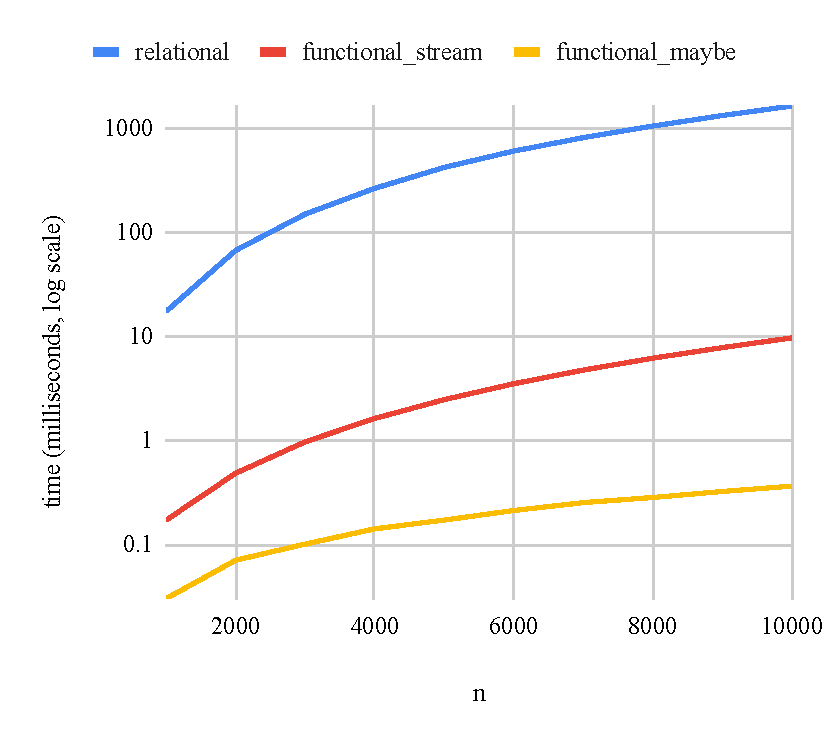
\includegraphics[height=0.85\textheight]{figures/maybe.pdf}
  \end{center}
\end{frame}

\begin{frame}[fragile]
  \frametitle{Need for Determinism Check}
\begin{center}
  Simply replacing the type of monad from \texttt{Stream} to \texttt{Maybe} improves performance 10 times for~relations on natural numbers
\end{center}

\begin{center}
  Pure (no monad) version is even faster
\end{center}

\vfill

\begin{center}
  Use determinism check to figure out when replacing \texttt{Stream} is feasible
\end{center}

\end{frame}

\begin{frame}[fragile]
  \frametitle{Need for Partial Deduction}

\begin{center}
Running a relational interpreter backwards fixes some arguments
\end{center}

\begin{center}
\begin{minipage}{0.3\textwidth}
  \lstinline{run q (eval$^o$ q true)}
\end{minipage}

\vfill

\begin{center}
  Augmenting functional conversion with partial deduction must be beneficial
\end{center}
\end{center}


\end{frame}


\begin{frame}[fragile]
  \frametitle{Conclusion}
Conclusion
  \begin{itemize}
    \item We presented a functional conversion scheme
    \item The conversion speeds up implementations considerably
    \item We implemented the conversion scheme in Haskell
    \item We found some way to order conjuncts
  \end{itemize}

\vfill

We are currently working on
  \begin{itemize}
    \item Determinism check
    \item Integration with partial deduction
    \item Integration into the framework of using relational interpreters for solving
  \end{itemize}
\end{frame}

\appendix
\backupbegin

\begin{frame}[fragile]
  \frametitle{Relational Sort}
\begin{columns}
  \begin{column}[t]{0.49\textwidth}
    
\lstset{moredelim=[is][\bfseries]{[*}{*]}}

\begin{figure}[h]
  \centering
  \begin{minipage}{0.65\columnwidth}
    \begin{lstlisting}[frame=tb,language=ocanren1]
 let rec sort$^o$ x y =
   (x === [] /\ y === []) \/ 
   (fresh (s xs xs$_1$)
     y === s :: xs$_1$ /\
     smallest$^o$ x s xs /\
     sort$^o$ xs xs$_1$)
    \end{lstlisting}
  \end{minipage}
\end{figure}


    \vfill

    \begin{center}
      Only good for sorting:

      \lstinline{run q (sort$^o$ xs q)}
    \end{center}

  \end{column}
  \begin{column}[t]{0.49\textwidth}
    \begin{figure}[h]
  \centering
  \begin{minipage}{0.87\columnwidth}
    \begin{lstlisting}[frame=tb]
 let rec sort$^o$ x y = conde [
    (x === [] /\ y === []);
    (fresh (s xs xs$_1$)
      y === s :: xs$_1$ /\
      [*sort$^o$ xs xs$_1$ /\
      smallest$^o$ x s xs)*]]
    \end{lstlisting}
  \end{minipage}
\end{figure}


    \vfill

    \begin{center}
      Only good permutation generation:

      \lstinline{run q (sort$^o$ q xs)}
    \end{center}


  \end{column}
\end{columns}
\end{frame}

\begin{frame}[fragile]
  \frametitle{Relational Sort: Sorting}

\begin{table}[]
\begin{tabular}{l||c|r||r}
                & \multicolumn{2}{c||}{Relation} & \multicolumn{1}{c}{\multirow[t]{2}{*}{Function}} \\ \cline{2-3}
                & \multicolumn{1}{l|}{\begin{tabular}[c]{@{}l@{}}\texttt{sorto}\\ \texttt{smallesto}\end{tabular}} & \multicolumn{1}{l||}{\begin{tabular}[c]{@{}l@{}}\texttt{smallesto}\\ \text{sorto}\end{tabular}} & \multicolumn{1}{c}{}                            \\ \hline
\texttt{{[}3;2;1;0{]}}   & \multicolumn{1}{r|}{0.077s}                                                    & 0.004s                                                                         & 0.000s                                          \\
\texttt{{[}4;3;2;1;0{]}} & timeout                                                                       & 0.005s                                                                         & 0.000s                                          \\
\texttt{{[}31;...;0{]}}  & timeout                                                                       & 1.058s                                                                         & 0.006s                                          \\
\texttt{{[}262;...;0{]}} & timeout                                                                       & \multicolumn{1}{c||}{timeout}                                                   & 1.045s
\end{tabular}
\end{table}

\end{frame}


\begin{frame}[fragile]
  \frametitle{Relational Sort: Generating Permutations}

\begin{table}[]
\begin{tabular}{l||c|r||r}
                & \multicolumn{2}{c||}{Relation} & \multicolumn{1}{c}{\multirow[t]{2}{*}{Function}} \\ \cline{2-3}
                & \multicolumn{1}{l|}{\begin{tabular}[c]{@{}l@{}}\texttt{smallesto}\\ \texttt{sorto}\end{tabular}} & \multicolumn{1}{l||}{\begin{tabular}[c]{@{}l@{}}\texttt{sorto}\\ \text{smallesto}\end{tabular}} & \multicolumn{1}{c}{}                            \\ \hline
\texttt{{[}0;1;2{]}}   & \multicolumn{1}{r|}{0.013s}                                                    & 0.004s                                                                         & 0.004s                                          \\
\texttt{{[}0;1;2;3{]}} & timeout                                                                       & 0.005s                                                                         & 0.005s                                          \\
\texttt{{[}0;...;6{]}}  & timeout                                                                       & 0.999s                                                                         & 0.021s                                          \\
\texttt{{[}0;...;8{]}} & timeout                                                                       & \multicolumn{1}{c||}{timeout}                                                   & 1.543s
\end{tabular}
\end{table}

\end{frame}

\backupend

\end{document}
